\begin{figure}[H]
    \centering
    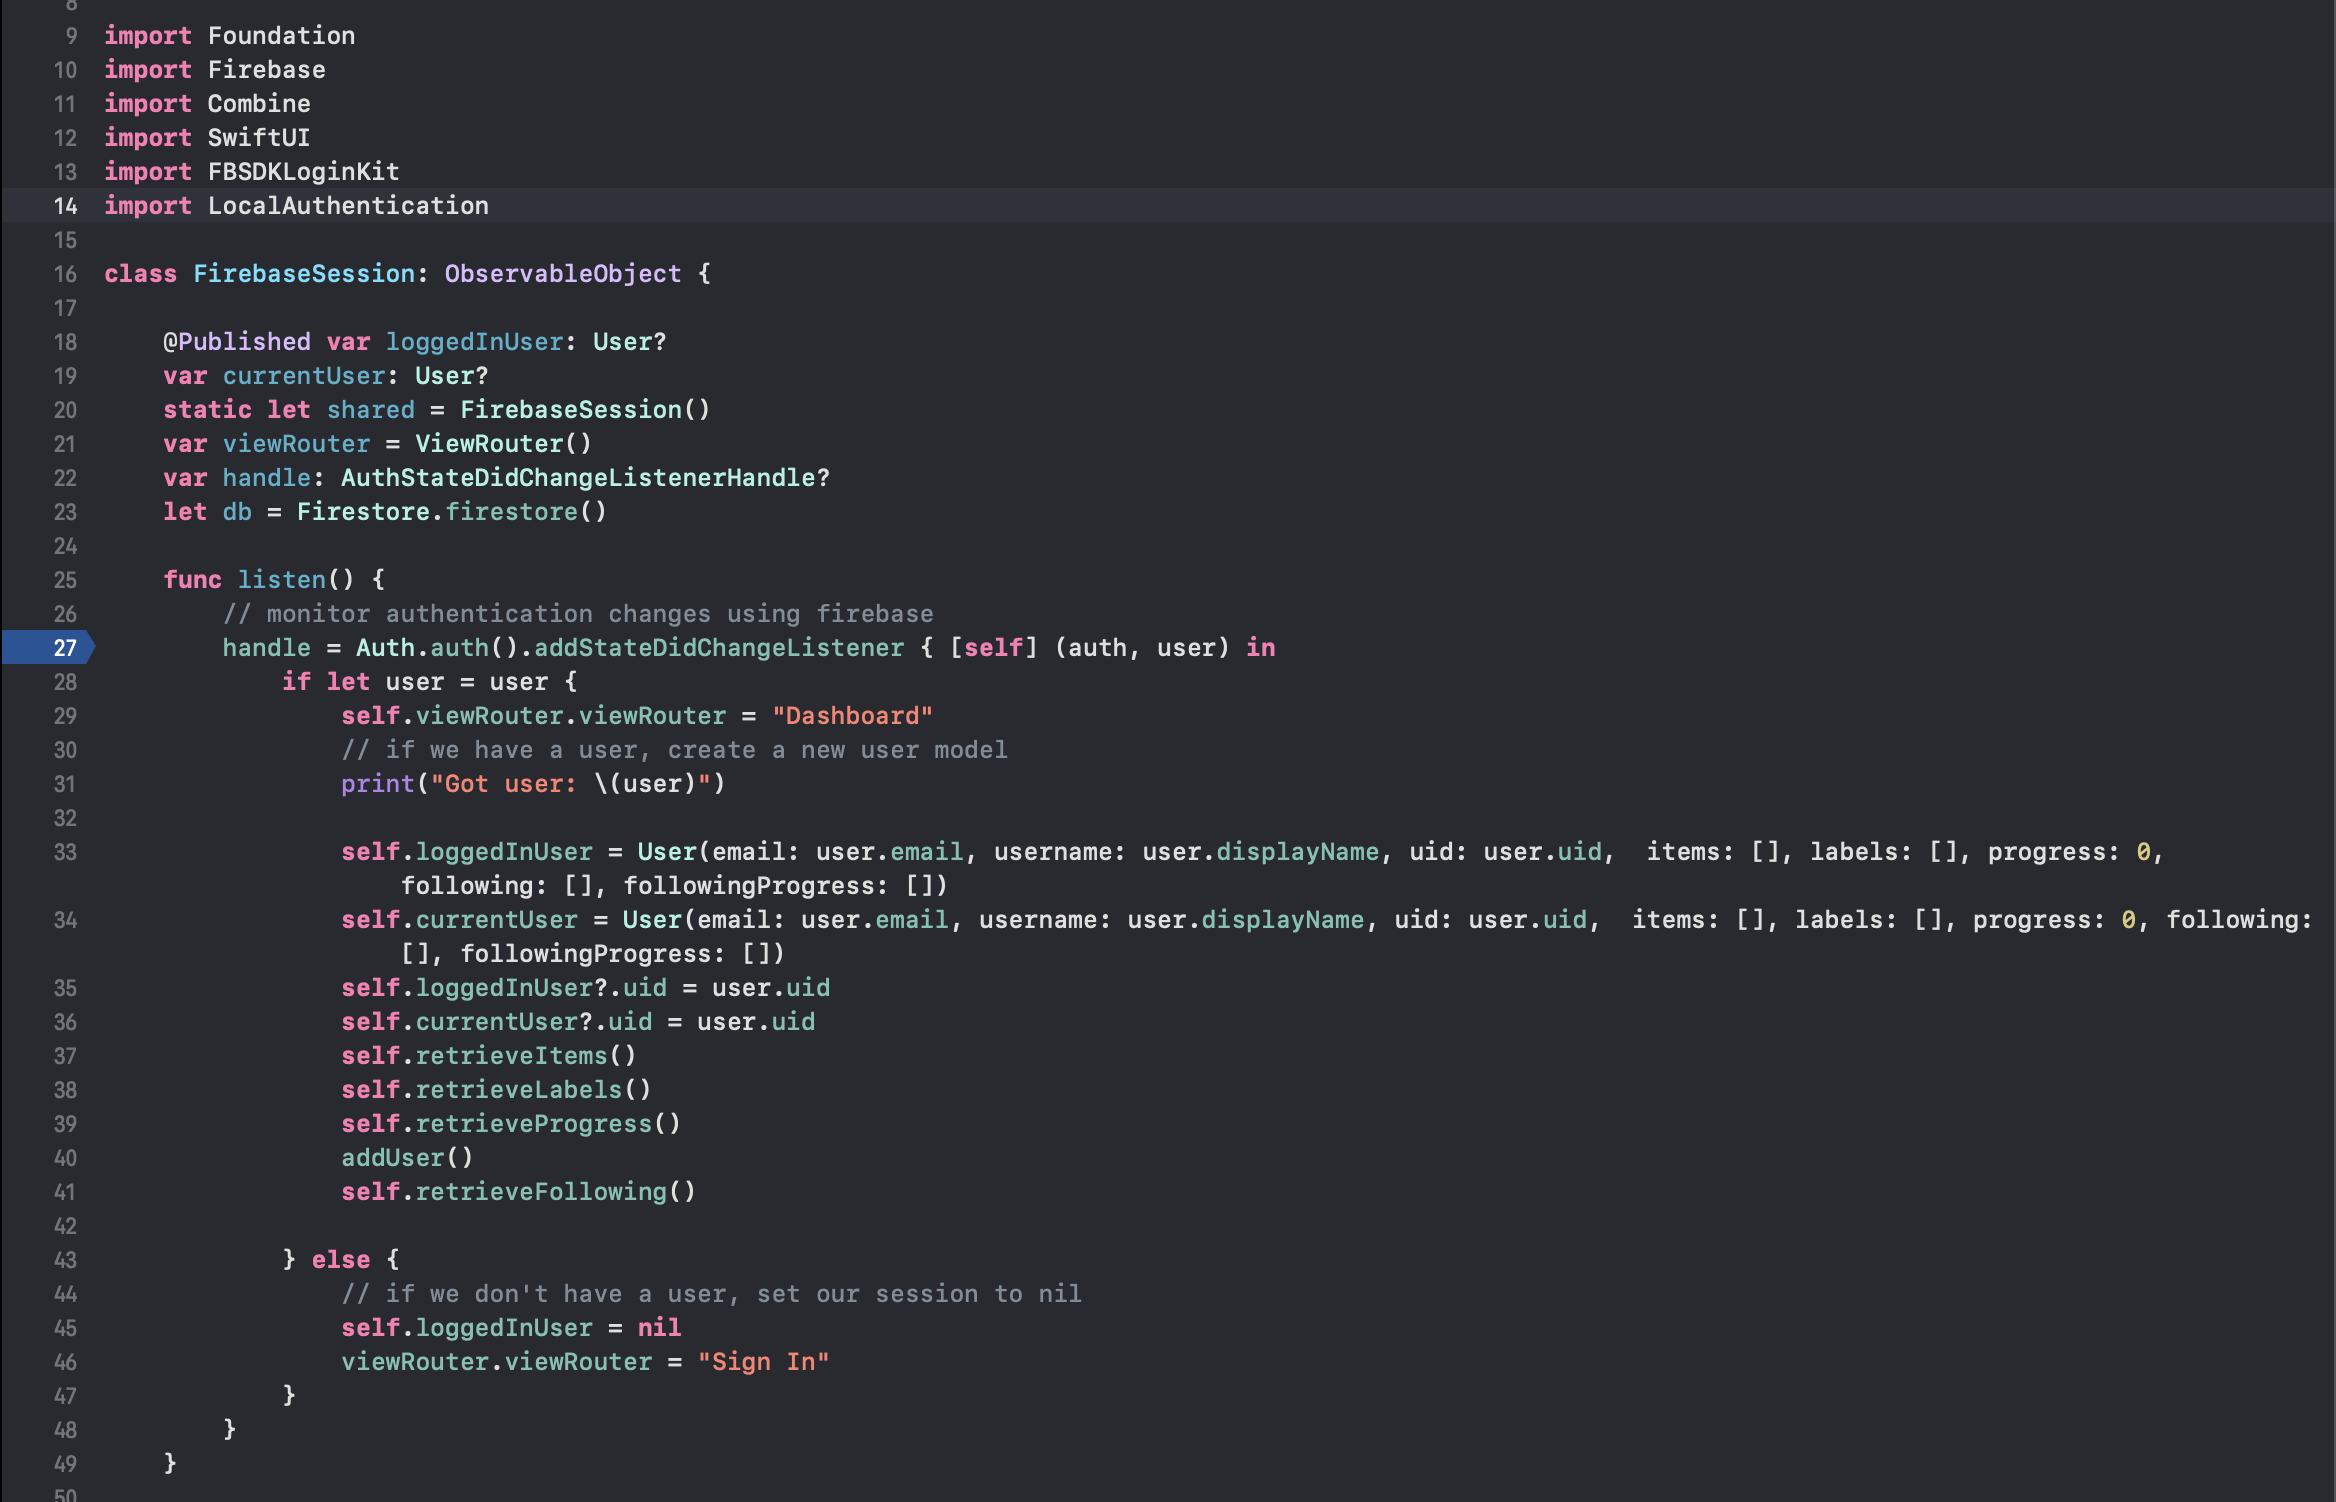
\includegraphics[width=\textwidth]{./graphics/Implementation/Splash_Sign_Up_Sign_In/firebasesession1.png}
    \caption{Global variables and listen() function defined in the FirebaseSession class.}
    \label{fig:firebasesession1}
\end{figure}

\begin{figure}[H]
    \centering
    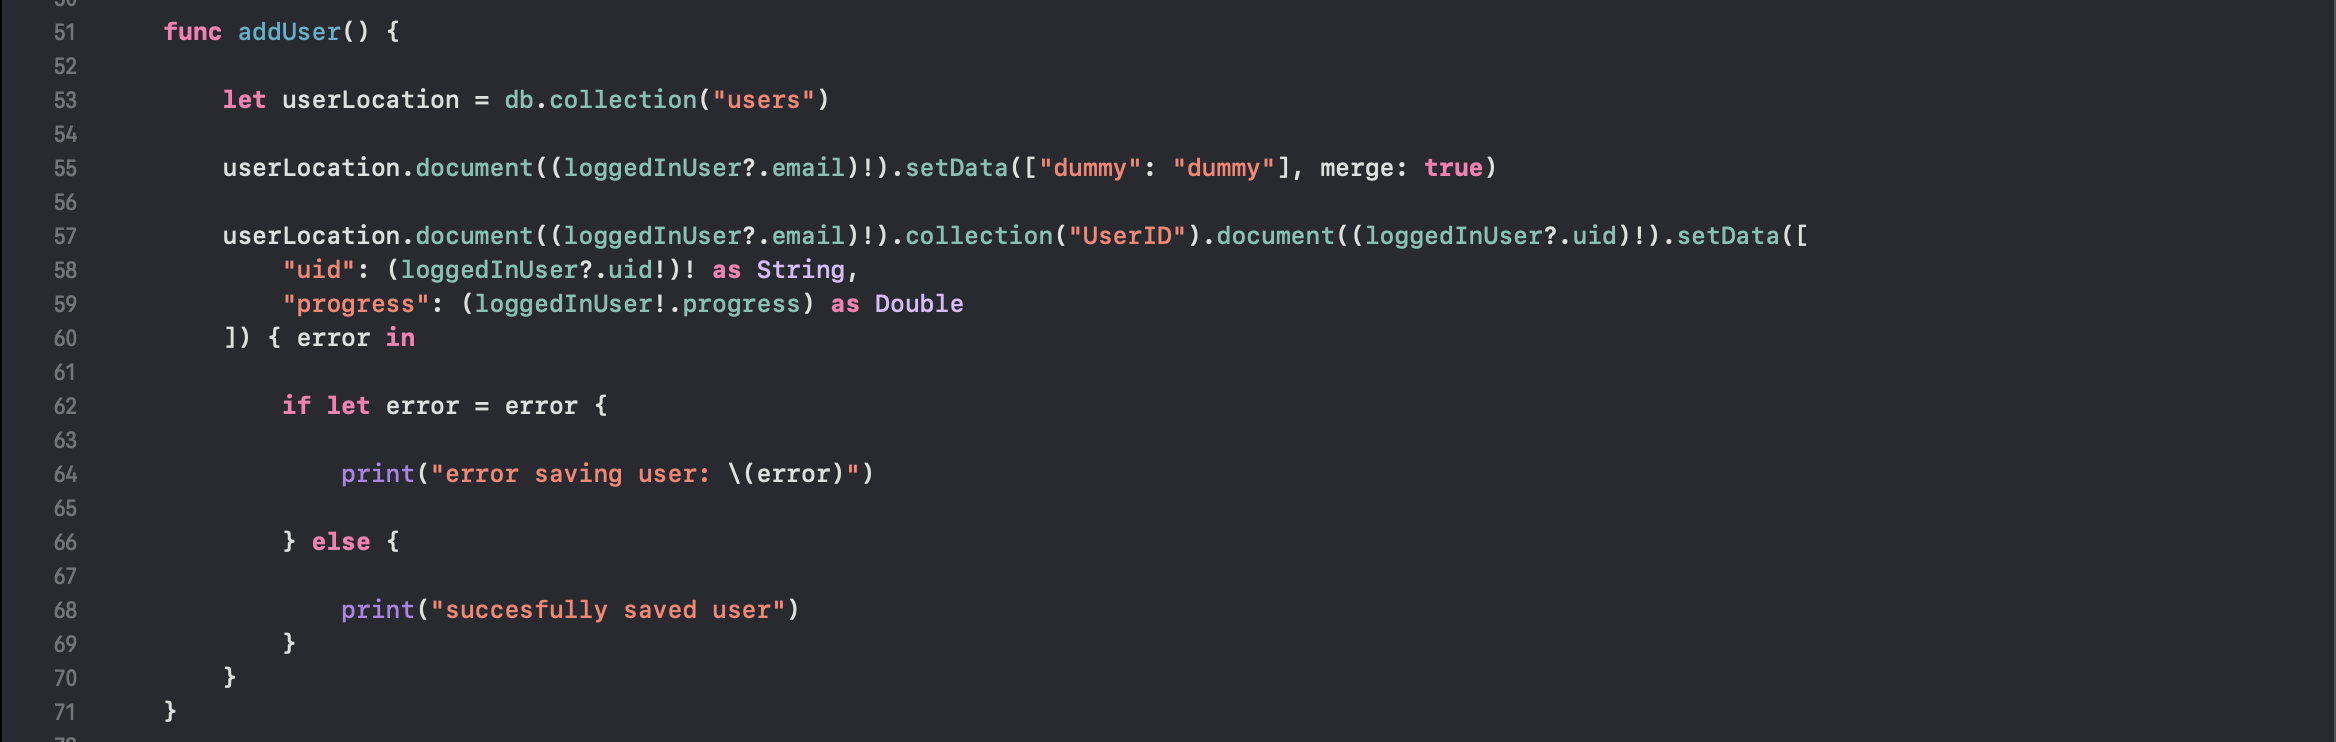
\includegraphics[width=\textwidth]{./graphics/Implementation/Splash_Sign_Up_Sign_In/firebasesession2.png}
    \caption{addUser() function defined in the FirebaseSession class.}
    \label{fig:firebasesession2}
\end{figure}

\begin{figure}[H]
    \centering
    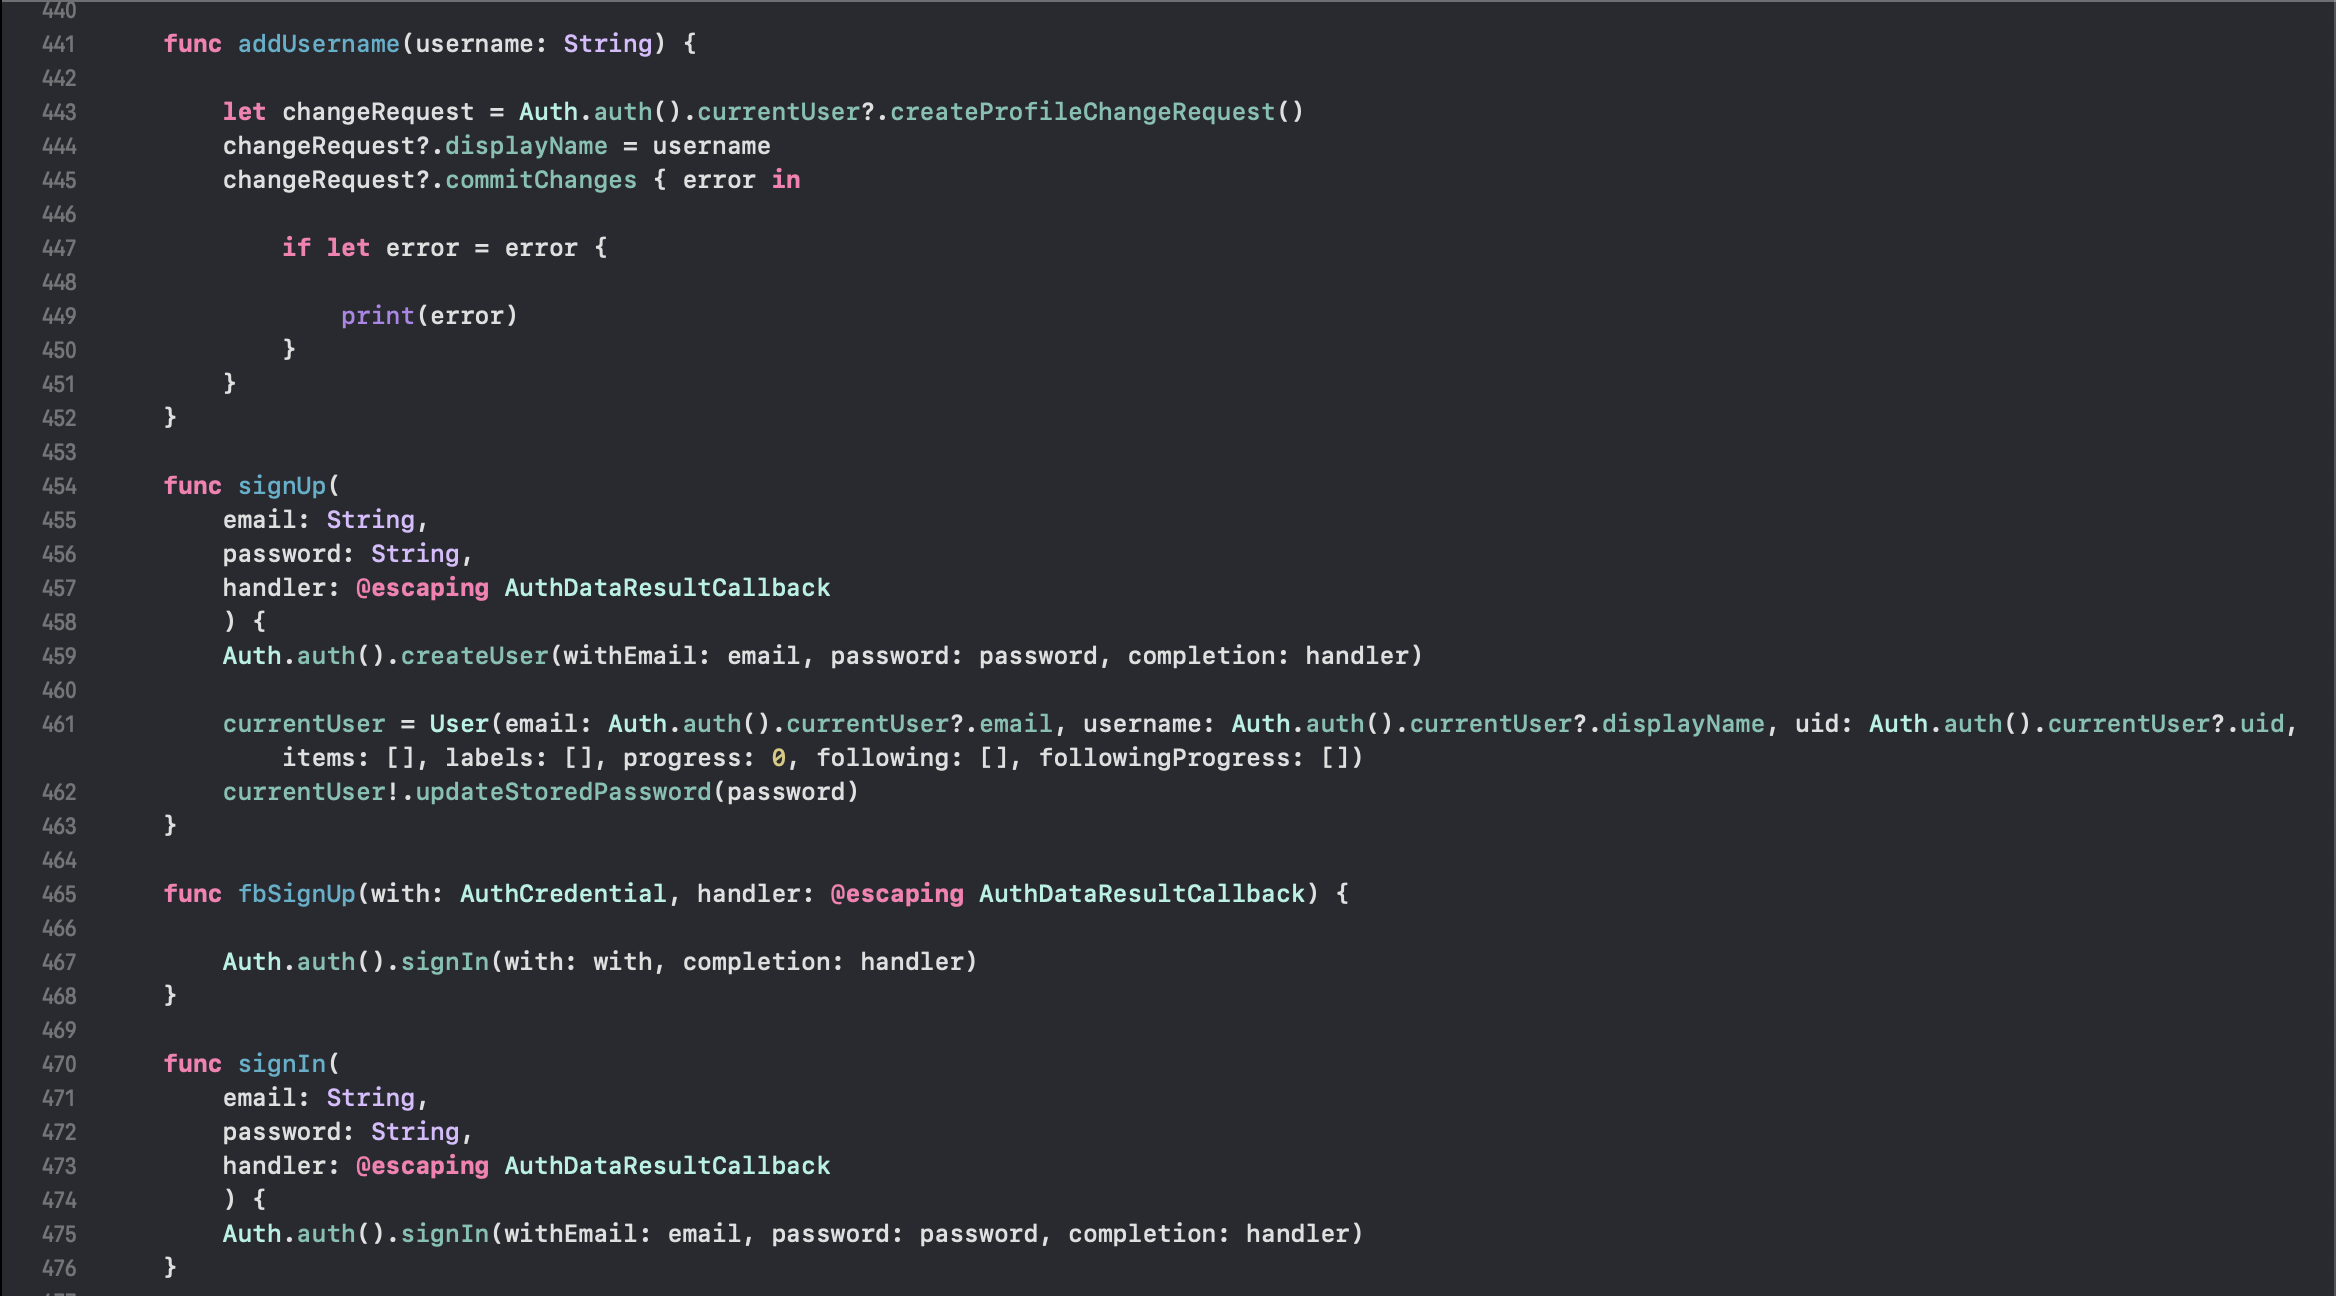
\includegraphics[width=\textwidth]{./graphics/Implementation/Splash_Sign_Up_Sign_In/firebasesession3.png}
    \caption{addUsername(), signUp(), fbSignUp() and signIn() functions defined in the FirebaseSession() class.}
    \label{fig:firebasesession3}
\end{figure}

\begin{figure}[H]
    \centering
    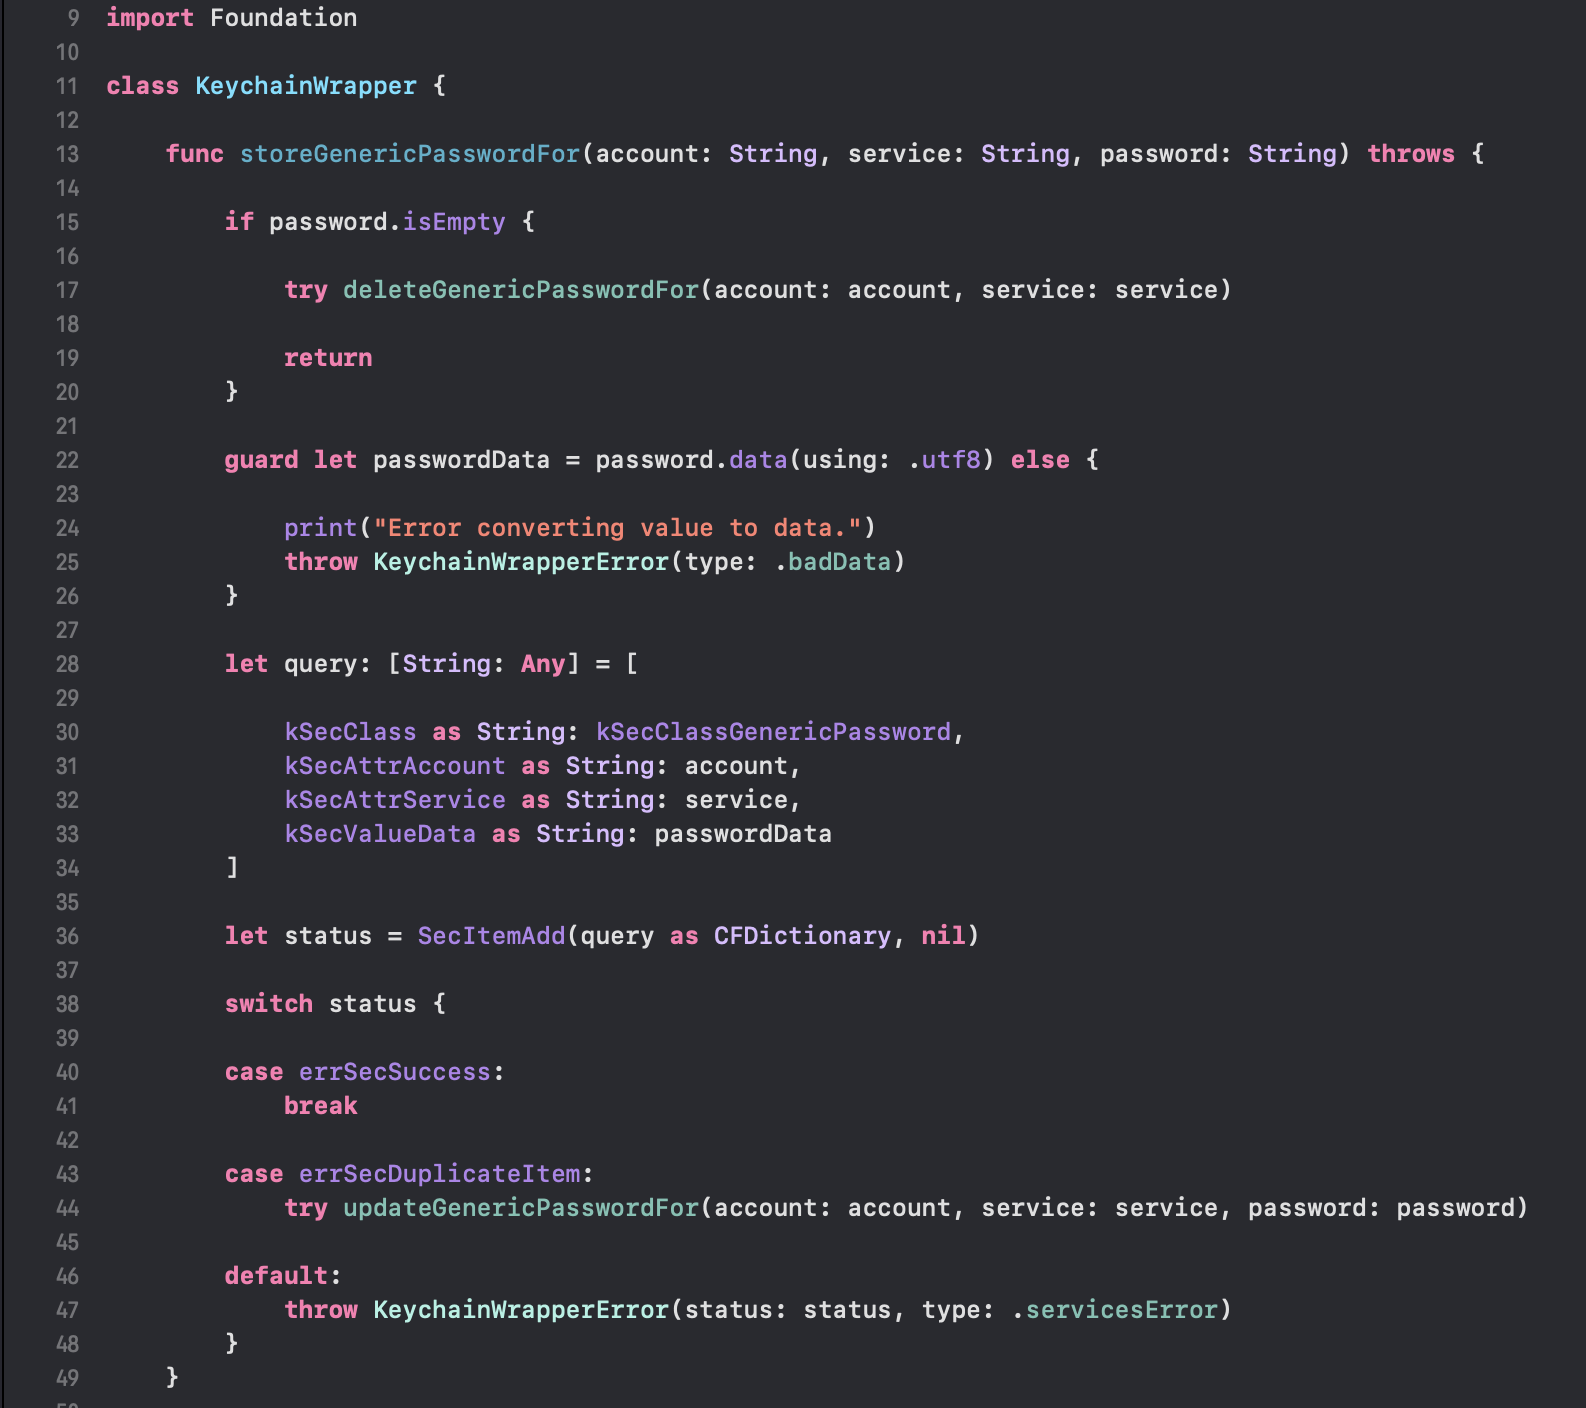
\includegraphics[width=\textwidth]{./graphics/Implementation/Settings/keychain1.png}
    \caption{storeGenericPasswordFor() function in the KeychainWrapper class.}
    \label{fig:keychain1}
\end{figure}

\begin{figure}[H]
    \centering
    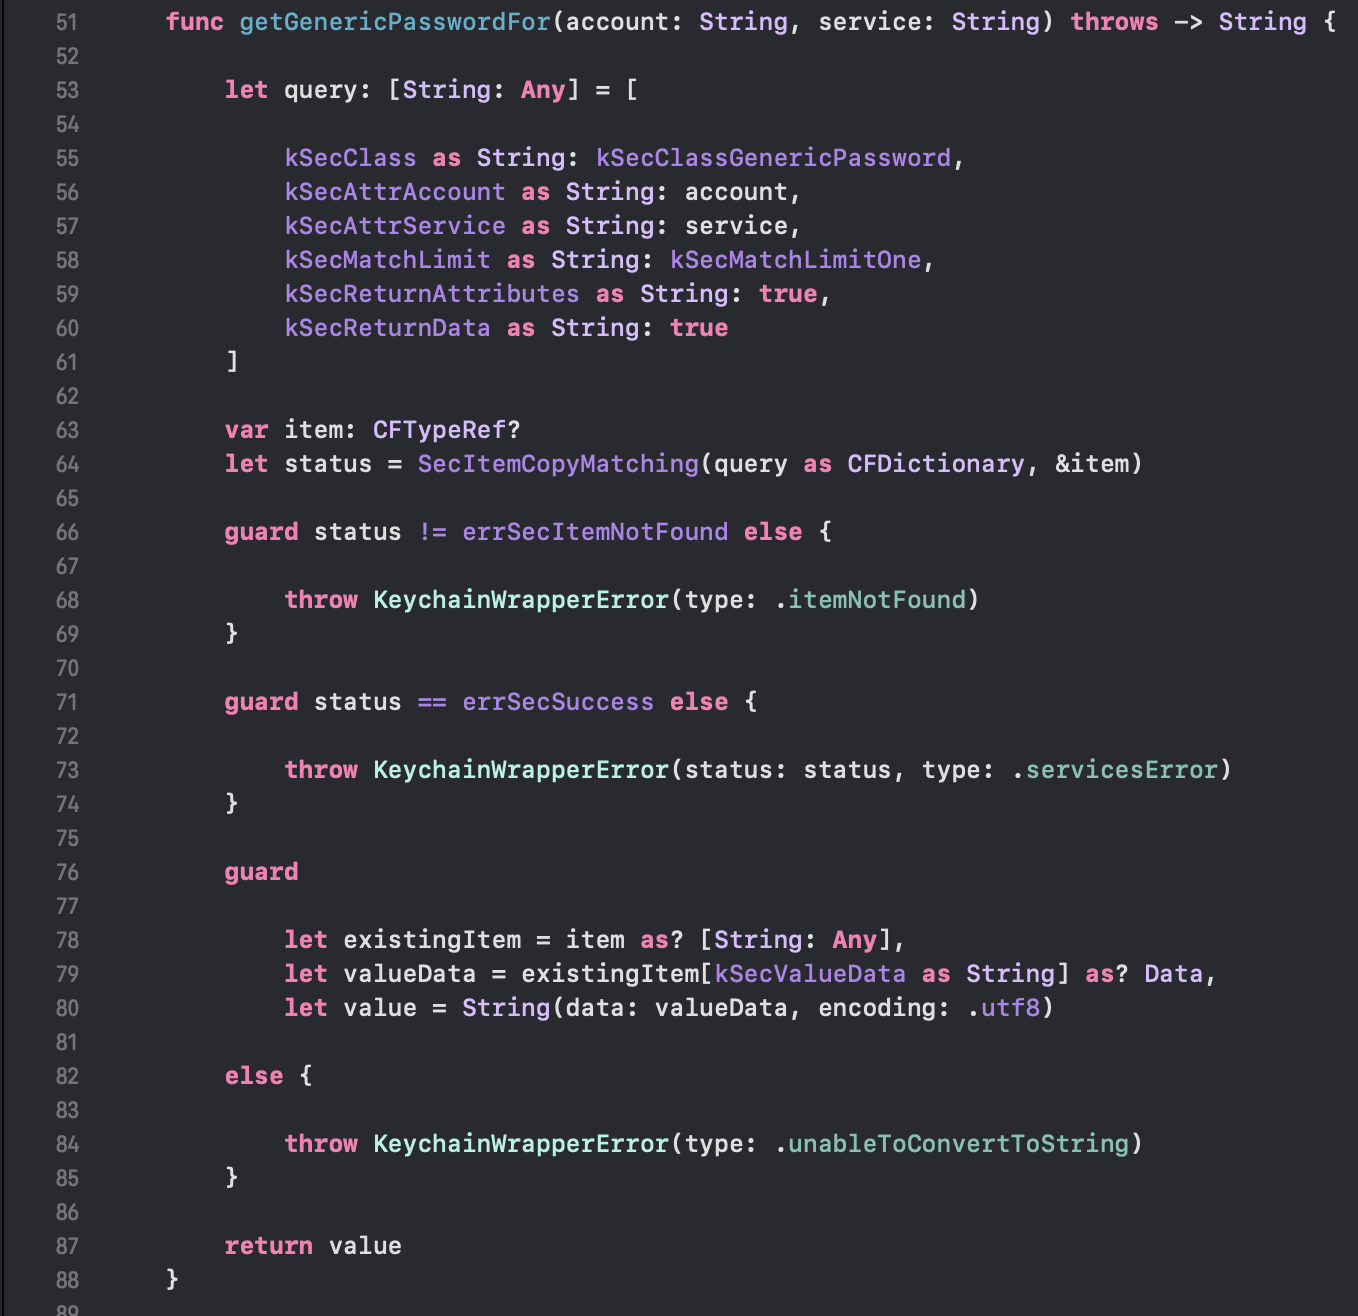
\includegraphics[width=\textwidth]{./graphics/Implementation/Settings/keychain2.png}
    \caption{getGenericPasswordFor() function in the KeychainWrapper class.}
    \label{fig:keychain2}
\end{figure}

\begin{figure}[H]
    \centering
    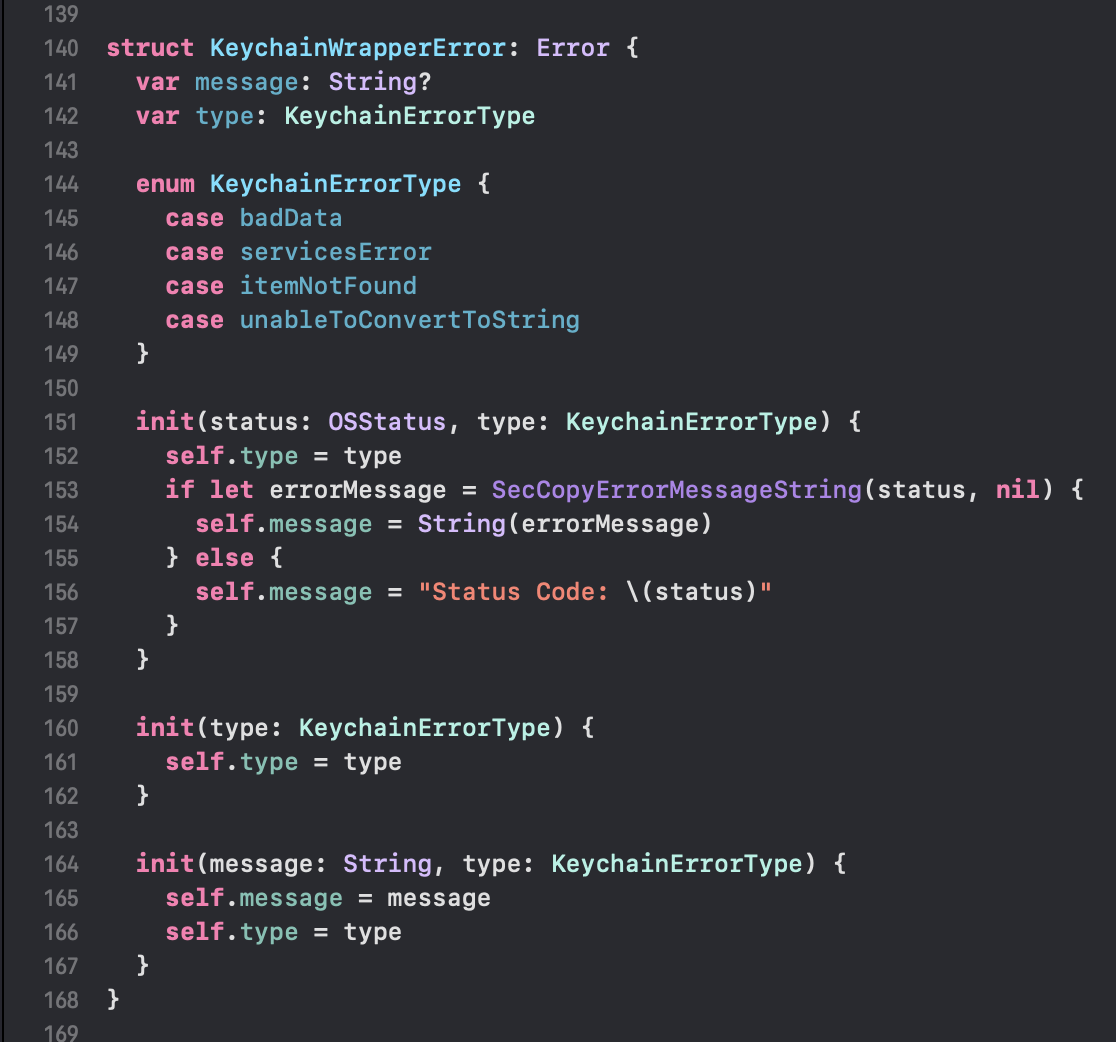
\includegraphics[width=\textwidth]{./graphics/Implementation/Settings/keychain5.png}
    \caption{KeychainWrapperError struct contained in the KeychainWrapper class.}
    \label{fig:keychain5}
\end{figure}